\documentclass[fleqn,10pt]{physiome}
\usepackage{multirow}
\usepackage{mathtools}
\usepackage{listings}
\captionsetup[table]{name=Tabela}
\captionsetup[figure]{name=Rysunek}

% Use option lineno for line numbers 

\title{Interfejsy i Multimedia w Technice - Projekt}


\author[]{Maciej Miszczak, Dominik Trochowski}
\curator{M&D}
\begin{document}

\maketitle
\renewcommand{\abstractname}{Streszczenie}
\begin{abstract}
    Wykonanie projektu ramienia robota 2R, korzystając z języka programowania Python. Do realizacji zadania posłużono się gotowym przykładem opisującym problem podwójnego wahadła, który sukcesywnie modyfikowano do uzyskania satysfakcjonującego efektu. Modyfikacje polegały na kompletnej zmianie modelu matematycznego, implementacji regulatora PID oraz zmianach wizualnych w czasie animacji.
    \newline
    \newline
    Słowa kluczowe: Regulator PID, Manipulator, Podwójne wahadło.
\end{abstract}



\section{Wstęp}
    Współcześnie można zaobserwować ciągły przyrost liczby występowania robotów w różnych dziedzinach przemysłu oraz  w życiu codziennym. Wykorzystanie robotów pozwala na zwiększenie wydajności produkcji oraz obniżenie jej kosztów. Z szeroko rozumianą robotyką powiązane jest m.in pojęcie manipulatora. Jest to mechanizm zastępujący czynności ruchowe człowieka, a dokładniej – realizujący niektóre funkcje kończyny górnej.
    Celem projektu jest zaprojektowanie ramienia robota R2, korzystając z języka programowania - Python. Jest to wysokopoziomowy język programowania ogólnego przeznaczenia zawierający rozbudowany pakiet bibliotek standardowych, którego ideą przewodnią jest czytelność i klarowność kodu źródłowego. Jego składnia cechuje się przejrzystością i zwięzłością.
	
   

\section{Cel projektu}
\begin{table}[ht]
\centering
\begin{tabular}{|c|c|}
\hline
Temat: Ramię robota w 2D (2 stopnie swobody)      & Numer zadania: R2      \\ \hline
\multicolumn{2}{|c|}{}                                                     \\ \hline
Zadanie                                           & Czas wykonania {[}h{]} \\ \hline
\multirow{3}{*}{Zbudowanie modelu matematycznego} & Czas minimalny: 1      \\ \cline{2-2} 
                                                  & Czas realny $\sim$2.5  \\ \cline{2-2} 
                                                  & Czas maksymalny: 5     \\ \hline
\multirow{3}{*}{Implementacja układu sterowania}  & Czas minimalny: 3      \\ \cline{2-2} 
                                                  & Czas realny: $\sim$5   \\ \cline{2-2} 
                                                  & Czas maksymalny: 12    \\ \hline
\multirow{3}{*}{Stworzenie animacji}              & Czas minimalny: 0.5    \\ \cline{2-2} 
                                                  & Czas realny: $\sim$1   \\ \cline{2-2} 
                                                  & Czas maksymalny: 2h    \\ \hline
\end{tabular}
\caption{\label{tab:widgets}Tabela z wymaganiami.}
\end{table}
\newpage
\section{Model matematyczny}

W realizacji modelu matematycznego dla projektowanego ramienia robota 2R szczególnie pomocnym okazał się rozdział drugi w artykule autorstwa Okubanjo, A. A.*, Oyetola, O. K., Osifeko, M. O., Olaluwoye, O. O. and Alao, P. O. pod tytułem "Modeling of 2 DOF Robot Arm and Control". Uzyskany model matematyczny jest widoczny poniżej:

\begin{equation}
    M(\Theta) \ddot{\Theta} + C(\Theta,\dot{\Theta}) \dot{\Theta} + G(\Theta) = \tau
\end{equation}
gdzie:
\newline
 $M(\Theta)$ - Macierz inercji,\newline
 $C(\Theta,\dot{\Theta})$ - Macierz związana z siłą odśrodkową oraz siłą Coriolisa,\newline
 $G(\Theta)$ - Wektor związany z siłą grawitacji,\newline
 $\tau$ - Macierz ze zmiennymi sterowanymi.(???)\newline
 \newline
 Składniki macierzy $M(\Theta)$:\newline
 \begin{equation}
     M(1,1)=(m_1+m_2) l_{1}^{2}+m_2l_{2}^{2}+2m_2l_1l_2cos(\Theta_2)
 \end{equation}
 \begin{equation}
     M(1,2)=m_2 l_{2}^{2}+m_2l_1l_2cos(\Theta_2)
 \end{equation}
 \begin{equation}
     M(2,1)=m_2 l_{2}^{2}+m_2l_1l_2cos(\Theta_2)
 \end{equation}
 \begin{equation}
     M(2,2)=m_2 l_{2}^{2}
 \end{equation}
 \newline
 Składniki macierzy $C(\Theta,\dot{\Theta})$:
 \newline
  \begin{equation}
     C(1,1)=0
 \end{equation}
 \begin{equation}
     C(1,2)=-2m_2l_1l_2sin(\Theta_2)\dot{\Theta_1}\dot{\Theta_2}-m_2l_1l_2sin(\Theta_2)\dot{\Theta_{2}^{2}}   
 \end{equation}
 \begin{equation}
     C(2,1)=m_2l_1l_2sin(\Theta_2)\dot{\Theta_{1}^{2}}
 \end{equation}
 \begin{equation}
     C(2,2)=0
 \end{equation}
  \newline
 Składniki wektora $G(\Theta)$:
\newline
\begin{equation}
     G(1,1)=(m_1+m_2)gl_1sin(\Theta_1)+m_2gl_2sin(\Theta_1+\Theta_2)
\end{equation}
\begin{equation}
     C(2,1)=m_2gl_2sin(\Theta_1+\Theta_2)
\end{equation}
\newline
\section{Kod programu}
Program stworzony w języku programowania Python został przedstawiony poniżej:
\newline
\begin{lstlisting}[language=Python]
import math
from numpy import sin, cos
import numpy as np
import matplotlib.pyplot as plt
import scipy.integrate as integrate
import matplotlib.animation as animation

G = 9.8 # przyspieszenie ziemskie
L1 = 1.0 # dlugosc czlonu pierwszego
L2 = 1.0 # dlugosc czlonu drugiego
M1 = 1.0 # masa czlonu pierwszego
M2 = 1.0 # masa czlonu drugiego

Kp1 = 0.35 # wzmocnienie czlonu proporcjonalnego przegub 1
Ki1 = 0.05 # wzmocnienie czlonu calkujacego przegub 1
Kd1 = 0.008 # wzmocnienie czlonu rozniczkujacego przegub 1

Kp2 = 0.38 # wzmocnienie czlonu proporcjonalnego przegub 2
Ki2 = 0.2 # wzmocnienie czlonu calkujacego przegub 2
Kd2 = 0.0001 # wzmocnienie czlonu rozniczkujacego przegub 2

th1_ = 25.0 # wartosc zadana kata przegubu pierwszego (stopnie)
th2_ = 25.0 # wartosc zadana kata przegubu drugiego (stopnie)

th1_r = np.radians(th1_)
th2_r = np.radians(th2_)

e1 = 0.0 # wartosc uchybu regulacji przegubu pierwszego
e2 = 0.0 # wartosc uchybu regulacji przegubu drugiego

uchyb_poprzedni1 = 0.0 # zmienna buforu uchybu pierwszego
uchyb_poprzedni2 = 0.0 # zmienna buforu uchybu drugiego

def derivs(state, t):

dydx = np. zeros_like(state)
# regulator PID przegubu pierwszego
e1 = th1_ - state[0]
pochodna1 = (e1 - uchyb_poprzedni1)/dt
sterowanie1 = Kp1*e1  + Ki1*dydx[4] + Kd1*pochodna1
uchyb_poprzedni_1 = e1

# regulator PID przegubu drugiego
e2 = th2_ - state[2]
pochodna2 = (e2 - uchyb_poprzedni2)/dt
sterowanie2 = Kp2*e2 + Ki2*dydx[5] + Kd2*pochodna2
uchyb_poprzedni_2 = e2
    
suma = state[0] + state[2]
    
M11 = (M1 + M2)*L1**2 + M2*L2**2 + 2*M2*L1*L2*cos(state[2])
M12 = M2*L2**2 + M2*L1*L2*cos(state[2])
M21 = M2*L2**2 + M2*L1*L2*cos(state[2])
M22 = M2*L2**2

C12 = -2*M2*L1*L2*sin(state[2])*state[1]*state[3]
- M2*L1*L2*sin(state[2])*state[3]*state[3]
C21 = M2*L1*L2*sin(state[2])*state[1]*state[1]

G11 = (M1+M2)*G*L1*sin(state[0]) + M2*G*L2*sin(suma)
G21 = M2*G*L2*sin(suma)

den = M11*M22 - M12*M21
    
dydx[0] = state[1]

dydx[1] = ((+ M22*(sterowanie1 - C12*state[3] - G11)
- M12*(sterowanie2 - C21*state[1] - G21))/den)
    
dydx[2] = state[3]

dydx[3] = ((- M21*(sterowanie1 - C12*state[3] - G11)
+ M11*(sterowanie2 - C21*state[1] - G21))/den)

dydx[4] = e1

dydx[5] = e2
return dydx


# tworzenie tablicy czasu od 0..100 probkowanej co 0.05 sekundy
dt = 0.05
t = np.arange(0, 40, dt)

# th1 i th2 sa poczatkowymi katami (stopnie)
# w1 i w2 sa poczatkowymi predkosciami katowymi (stopnie na sekunde)
th1 = 0.0
w1 = 0.0
th2 = 0.0
w2 = 0.0

# stan poczatkowy
state = np.radians([th1, w1, th2, w2, e1, e2])

# integrate your ODE using scipy.integrate.
y = integrate.odeint(derivs, state, t)

x1 = L1*sin(y[:, 0])
y1 = -L1*cos(y[:, 0])

x2 = L2*sin(y[:, 2]) + x1
y2 = -L2*cos(y[:, 2]) + y1

x1z = L1*sin(th1_r)
x2z = L2*sin(th2_r)+x1z

y1z = -L1*cos(th1_r)
y2z = -L2*cos(th2_r)+y1z


fig = plt.figure()
ax = fig.add_subplot(111, autoscale_on=False, xlim=(-2, 2), ylim=(-2, 2))
ax.set_aspect('equal')
ax.grid()

line, = ax.plot([], [], 'o-', lw=2)
time_template = 'time = %.1fs'
time_text = ax.text(0.05, 0.9, '', transform=ax.transAxes)

zadana1, = ax.plot([], [], 'g', lw=2)
zadana1.set_data([0,x1z], [0,y1z])

zadana2, = ax.plot([], [], 'r', lw=2)
zadana2.set_data([x1z,x2z], [y1z,y2z])

def init():
    line.set_data([], [])
    time_text.set_text('')
    return line, time_text


def animate(i):
    thisx = [0, x1[i], x2[i]]
    thisy = [0, y1[i], y2[i]]

    line.set_data(thisx, thisy)
    time_text.set_text(time_template % (i*dt))
    return line, time_text


ani = animation.FuncAnimation(fig, animate, range(1, len(y)),
                              interval=dt*1000, blit=True, init_func=init)
plt.show()


\end{lstlisting}
\newpage
\section{Animacja}
Na poniższym rysunku przedstawiony został fragment animacji tworzonej przez kod programu.
\newline
\begin{figure}[ht]
\centering
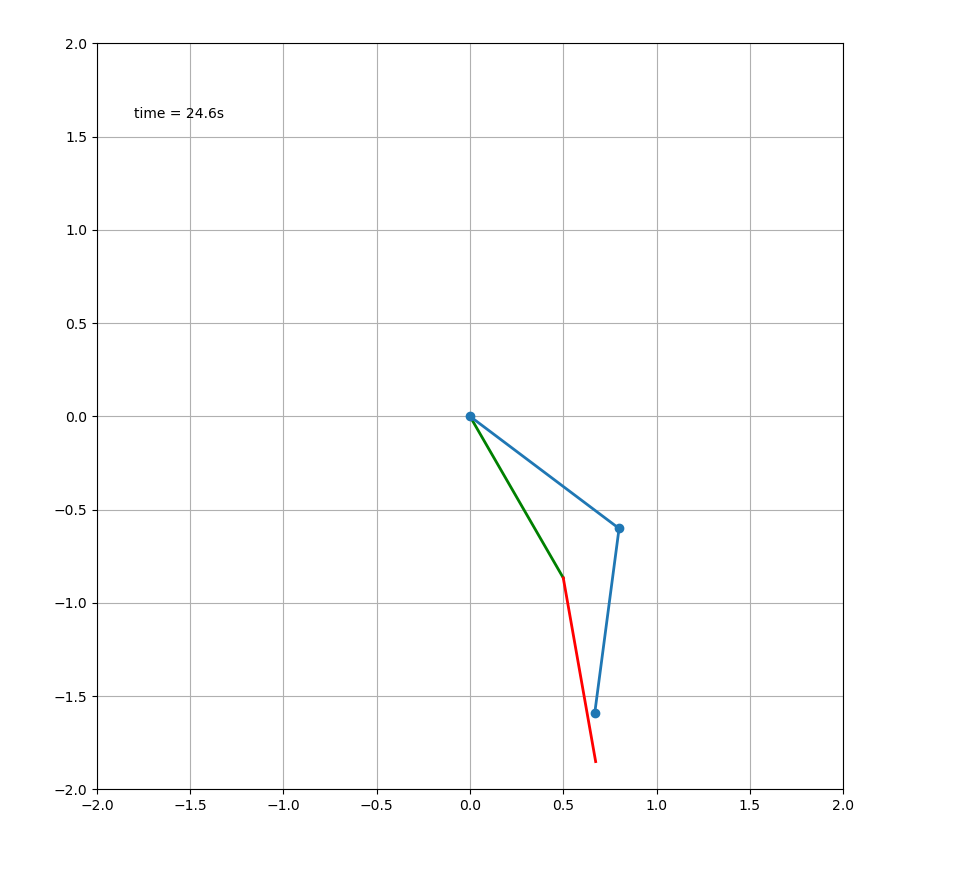
\includegraphics[width=0.8\linewidth]{zdjecie_monitory.PNG}
\caption{Fragment animacji ramienia robota 2R}
\label{fig:view}
\end{figure}
\newline
W lewym górnym rogu animacji został przedstawiony czas trwania animacji. Linie zielona oraz czerwona prezentują wartości zadane do jakich zmierzają wartości mierzone, prezentowane liniami niebieskimi. W przypadku prezentowanej animacji wartościami zadanymi kątów odchylenia są odpowiednio dla pierwszego członu: 30 stopni i dla drugiego członu: 10 stopni.

\section{Literatura}
Okubanjo, A. A.*, Oyetola, O. K., Osifeko, M. O., Olaluwoye, O. O. and Alao, P. O. "Modeling of 2 DOF Robot Arm and Control" Futo Journal Series (FUTOJNLS)
e-ISSN : 2476-8456 p-ISSN : 2467-8325
Volume-3, Issue-2, pp- 80 - 92
www.futojnls.org


\end{document}